% !TEX encoding = UTF-8
% !TEX TS-program = pdflatex
% !TEX root = ../tesi.tex
% !TEX spellcheck = it-IT

%**************************************************************
%taken from http://speect.sourceforge.net/topics/introduction_topic.html
\chapter{Speect}
\label{cap:speect}
%**************************************************************

\intro{\textbf{Speect} è un sistema di \textit{TTS} suddivisibile logicamente in un \textit{engine} principale e nei \textit{plug-in}. 
L'\textit{engine} è generico e completamente indipendente da qualsiasi modulo di \textit{text-to-speech}, occupandosi esclusivamente 
del caricamento di voci, \textit{plug-in} e dati, e del controllo del processo di sintesi.} \\


%**************************************************************
%**************************************************************
\section{Visione ad alto livello del sistema}
Il processo di sintesi ha come elemento centrale la \textit{utterance}, illustrata in \hyperref[subsec:utterance]{sezione 3.1.1}, 
che viene processata da una \textit{voce}, 
descritta in \hyperref[subsec:voice]{sezione 3.1.5}, in accordo ad un \textit{utterance type} che definisce le operazioni 
da effettuare per portare a termine la sintesi, 
come descritto in \hyperref[subsec:utttype]{sezione 3.1.3}. Le varie operazioni necessarie vengono svolte utilizzando \textit{plug-in} 
specifici che implementano le varie componenti, illustrate in \hyperref[subsec:uttproc]{sezione 3.1.2} e \hyperref[subsec:featproc]{sezione 3.1.4}.
   \subsection{Utterance}
   \label{subsec:utterance}
   In linguistica una \textit{utterance} è l'unità più piccola di parlato, ossia una singola emissione di voce. \\
   In \textbf{Speect} lo stesso termine rappresenta la singola unità di parlato, nel senso di singola unità di analisi del testo
   e sintesi vocale; praticamente costituisce sia tutti i passaggi che servono a generare una singola emissione vocale a partire
   da un testo, sia l'\textit{input} e i risultati intermedi dell'elaborazione. \\
   Essa costituisce sia l'\textit{input} sia l'\textit{output} di tutti i processi del sistema,
   dal \textbf{NLP} (\textit{Natural Language Processing}) al \textbf{DSP} (\textit{Digital Signal Processing}). \\
   Le \textit{utterance} vengono modellate internamente dal sistema come \textit{Heterogeneous Relation Graph} (struttura dati esposta
   in seguito),
   grafo al quale le varie parti del sistema aggiungono informazioni.
   \subsection{Utterance processor}
   \label{subsec:uttproc}
   Gli \textit{utterance processor} ricevono in \textit{input} una \textit{utterance} e la trasformano sulla base di
   alcuni parametri dell'\textit{input} stesso, quali: 
   \begin{itemize}
     \item la \texttt{tipologia dell'\textit{input}}: ad esempio, l'elaborazione di un messaggio contenuto in un \textit{email}
       richiede dei passaggi aggiuntivi rispetto all'elaborazione di un blocco di testo semplice;
     \item la \texttt{lingua}: un processo come la sillabificazione, ad esempio, può avvenire in modi completamente differenti
       a seconda delle lingue;
     \item la \texttt{voce}: le voci si differenziano per altezza, timbro, e altre proprietà.
   \end{itemize}
   \label{subsec:utttype}
   \subsection{Utterance type}
   Un \textit{utterance type} non è altro che un insieme di \textit{utterance processor} operanti in sequenza su una \textit{utterance}
   in \textit{input}.
   \subsection{Feature processor}
   \label{subsec:featproc}
   Gli \textit{utterance processor} fanno uso al loro interno dei \textit{feature processor}, i quali si occupano di estrarre 
   le \textit{feature} dalle unità individuali di una \textit{utterance}. \\ I \textit{feature processor} sono definiti tramite
   mappe chiave-valore, e sono invocati utilizzando i loro nomi.
  \subsection{Le voci in Speect}
  \label{subsec:voice}
  All'interno di \textbf{Speect} la voce definisce l'insieme di \textit{utterance type}, ossia, come si deduce dalla spiegazione precedente,
  la catena di \textit{utterance processor} utilizzati per la sintesi. \\ La voce definisce inoltre l'associazione chiave-valore per i
  \textit{feature processor} sfruttati dagli \textit{utterance processor}. Essa stabilisce inoltre i propri dati, siano essi
  linguistici (come gli insiemi di fonemi) o acustici. \\ La voce in \textbf{Speect} sfrutta i seguenti \textit{file}:
       \begin{itemize}
         \item un \textit{file} di configurazione obbligatorio chiamato \texttt{voice.json}, contenente sia i dati linguistici e acustici sulla voce, 
           sia gli \textit{utterance type} e le mappe dei \textit{feature processor};
         \item un \textit{file} di configurazione chiamato \texttt{phoneset.json} contenente alcuni dati utili alla classificazione dei fonemi,
           come i tratti distintivi delle consonanti o delle vocali;
         \item un \textit{file} chiamato \texttt{addendum.json};
         \item un \textit{file} chiamato \texttt{lexicon.json}.
       \end{itemize}
Esiste una \textit{directory} distinta con i \textit{file} di configurazione per ogni lingua, con una struttura simile alla seguente: \\
\begin{center}
\begin{forest}
 for tree={
    font=\ttfamily,
    grow'=0,
    child anchor=west,
    parent anchor=south,
    anchor=west,
    calign=first,
    edge path={
      \noexpand\path [draw, \forestoption{edge}]
      (!u.south west) +(7.5pt,0) |- node[fill,inner sep=1.25pt] {} (.child anchor)\forestoption{edge label};
    },
    before typesetting nodes={
      if n=1
        {insert before={[,phantom]}}
        {}
    },
    fit=band,
    before computing xy={l=15pt},
  }
[voices
  [voice-it
    [voice.json]
    [phoneset.json]
    [addendum.json]
    [lexicon.json]
  ]
  [voice-zu
    [voice.json]
    [phoneset.json]
    [addendum.json]
    [lexicon.json]
  ]
]
\end{forest}
\end{center}

\subsection{Struttura e funzionamento dei \textit{plug-in}}
La struttura fortemente modulare di \textbf{Speect} ha reso necessaria la definizione di un
\textit{layout} di \textit{directory} \textit{standard} al quale ogni \textit{plug-in} sviluppato per
questo sistema deve essere conforme. La struttura viene qui riportata: \\
%I \textit{plug-in} possono essere caricati a \textit{runtime} attraverso un gestore interno al sistema. \\
%Il gestore dei \textit{plug-in} ha il compito di cercare la libreria dinamica contenente il \textit{plug-in},
%di caricarlo e di eseguirne la funzione di registrazione. Nel caso in cui un \textit{plug-in} per funzionare
%dipenda da altri \textit{plug-in}, questi verranno caricati simultaneamente al \textit{plug-in} principale. \\
%Una volta terminato l'utilizzo del \textit{plug-in} il 
\begin{center}
\begin{forest}
 for tree={
    font=\ttfamily,
    grow'=0,
    child anchor=west,
    parent anchor=south,
    anchor=west,
    calign=first,
    edge path={
      \noexpand\path [draw, \forestoption{edge}]
      (!u.south west) +(7.5pt,0) |- node[fill,inner sep=1.25pt] {} (.child anchor)\forestoption{edge label};
    },
    before typesetting nodes={
      if n=1
        {insert before={[,phantom]}}
        {}
    },
    fit=band,
    before computing xy={l=15pt},
  }
[plug-in-name
  [AUTHORS
  %  [text1.1.1]
  %  [text1.1.2]
  %  [text1.1.3]
  ]
  [README
    %[text1.2.1]
    %[text1.2.2]
  ]
  [CMakeLists.txt]
  [Doxyfile]
  [cmake
     [sources.cmake]
  ]
  [src
     [source.h]
     [source.c]
     [plugin.c]
  ]
]
\end{forest}
\end{center}
In \textbf{Speect} il \textit{deployment} dei \textit{plug-in} avviene sotto forma di librerie dinamiche. \\
Le librerie dinamiche permettono molti dei vantaggi dei \textit{plug-in}, quali l' \hyperref[glo:hots]{\emph{hot swapping}\glsfirstoccur},
l'estensione sicura da parte di sviluppatori terzi (cioè la possibilità di aggiungere funzionalità senza modificare il \textit{core}
del sistema), e tempi di \textit{linking} più brevi. \\
Al momento del caricamento di un \textit{plug-in}, il \textit{plug-in manager} interno al sistema cerca il simbolo \texttt{s\_plugin\_init}
nel \textit{plug-in}. Questo è l'unico simbolo caricato dal \textit{plug-in manager}, pertanto deve essere definito da ogni \textit{plug-in}
che deve essere integrato nel sistema. \\ Nei paragrafi seguenti vengono descritti brevemente i ruoli dei \textit{file} presenti
nello scheletro di ogni \textit{plug-in}. \\
\paragraph{Il \textit{file} plugin.c}
Questo \textit{file} fornisce una semplice funzione che definisce il simbolo \texttt{s\_plugin\_init}.
Questa funzione è utilizzata immutata da tutti i \textit{plug-in} implementati.
\paragraph{I \textit{file} source.h e source.c}
Il \textit{template} fornisce degli scheletri per i file \textit{header} e sorgenti. Ogni classe implementata 
possiede due funzioni, rispettivamente di registrazione e di eliminazione, aventi i seguenti prototipi:
   \begin{itemize}
       \item \texttt{S\_LOCAL void s\_classname\_reg(s\_erc *error)};
       \item \texttt{S\_LOCAL void s\_classname\_free(s\_erc *error)}.
   \end{itemize}
In \hyperref[app:appb]{Appendice B} vengono riportati alcuni frammenti di codice appartenenti
al \textit{template} comune a tutti i \textit{plug-in} di \textbf{Speect}.
%**************************************************************
\newpage

\begin{figure}[!h] 
    \centering 
    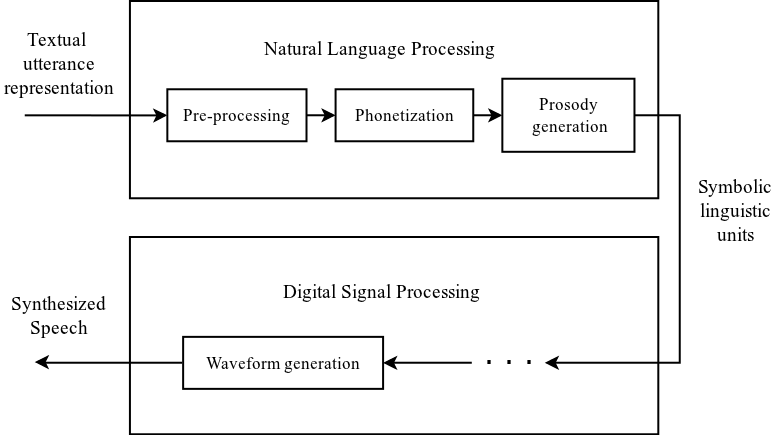
\includegraphics[width=0.9\columnwidth]{tts_con} 
    \caption{Componenti funzionali di un sintetizzatore}
\end{figure}

%**************************************************************

\section{Heterogeneous Relation Graph}
\subsection{Descrizione della struttura dati}
L'\textit{engine} di \textbf{Speect} rappresenta al suo interno l'\textit{utterance} tramite una struttura dati detta
\textbf{Heterogeneous Relation Graph} (HRG), ossia un grafo i cui nodi (detti \texttt{item}) sono organizzati per livelli
(detti \texttt{relation}). \\ Il sistema fornisce numerosi metodi per accedere al grafo e spostarsi all'interno dei suoi nodi,
anche attraverso le \textit{relation}. \\ Le \textit{relation} che costituiscono il grafo sono le seguenti:
\begin{itemize}
\item \texttt{Token}, è costituita da \textit{item} contenenti i \textit{token} dell'\textit{utterance};
\item \texttt{Word}: è costituita da \textit{item} contenenti le \textit{word} dell'\textit{utterance};
\item \texttt{Syllable}: è costituita da \textit{item} contenenti le sillabe che costituiscono le \textit{word};
\item \texttt{Segment}: è costituita da \textit{item} contenenti i fonemi delle \textit{word};
\item \texttt{SylStructure}: è una \textit{relation} che connette le tre \textit{relation} precedenti. \\
I nodi possono contenere anche informazioni aggiuntive chiamate \textit{feature}, calcolate dai \textit{feature processor}.
\end{itemize}

\subsection{Attraversamento del grafo}
Come si deduce dalla figura 3.2, le \textit{relation} \texttt{Word}, \texttt{Syllable} e \texttt{Segment} sono formate
da \textit{item} (tutti connessi) organizzati sotto forma di liste doppiamente concatenate attraversabili in entrambe le direzioni a partire da ogni nodo. \\
Dunque in queste tre \textit{relation} le uniche operazioni permesse per cambiare posizione rispetto ad un \textit{item} sono:
    \begin{enumerate}
      \item \texttt{next}: accesso all'\textit{item} successivo;
      \item \texttt{previous}: accesso all'\textit{item} precedente.
    \end{enumerate}
Diversamente dalle due \textit{relation} precedenti, la \textit{relation} \texttt{SylStructure}, come si vede dalla figura, 
non prevede che i suoi \textit{item} siano tutti connessi, ma fornisce altre due operazioni per la navigazione dei suoi nodi:
    \begin{enumerate}
      \item \texttt{daughter}: ogni \textit{item} può avere zero o più nodi figli;
      \item \texttt{parent}: ogni \textit{item} possiede uno e un solo nodo padre.
    \end{enumerate}

\subsection{Unicità degli item e condivisione del contenuto}
Gli \textit{item} sono univoci all'interno del grafo, tuttavia, nel caso in cui vi sia una sovrapposizione di contenuto tra 
due \textit{item} in due \textit{relation} distinte, questi sono considerati logicamente equivalenti. \\
In particolare, sempre facendo riferimento alla figura 3.2, si può notare come gli \textit{item} nella \textit{relation} \texttt{Word}
condividano il contenuto con gli \textit{item} al livello superiore della \textit{relation} \texttt{SylStructure}. Questa equivalenza
viene sfruttata per cambiare \textit{relation} durante l'attraversamento del grafo.

\begin{figure}[!h] 
    \centering 
    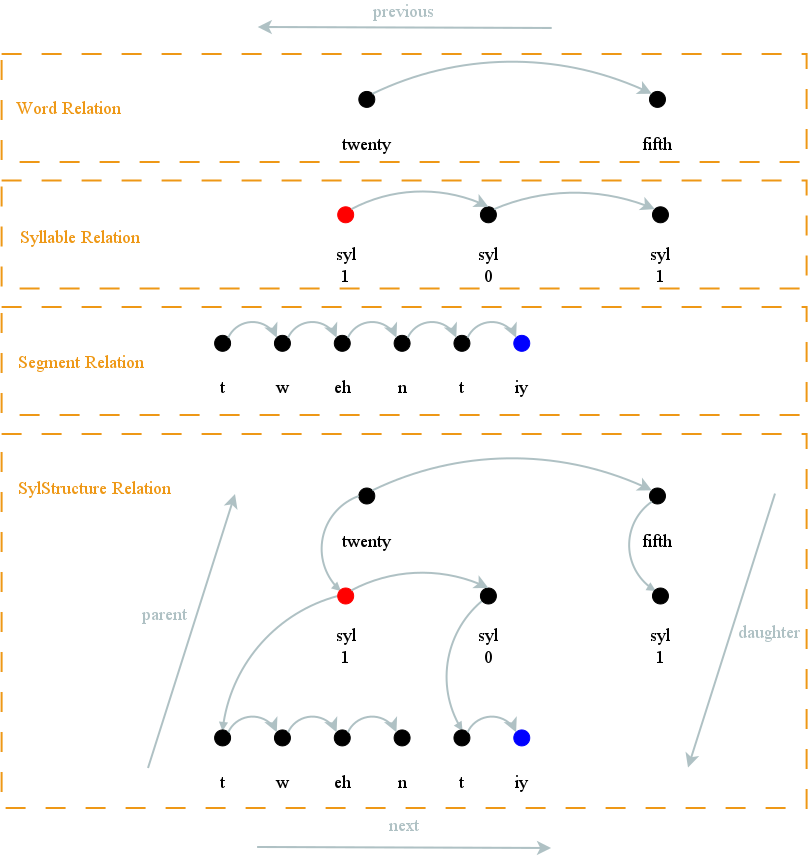
\includegraphics[width=0.9\columnwidth]{hrg} 
    \caption{Esempio di \textbf{H}eterogeneous \textbf{R}elation \textbf{G}raph}
\end{figure}



